\chapter{MOEA memético utilizando evolución diferencial}\label{diferencial}
\section{Introducción a la evolución diferencial}
\noindent A continuación se dará una breve introducción de la evolución diferencial
(\textit{Differential Evolution}, DE) \cite{Storn1997} para entender el algoritmo MPANN
(\textit{Memetic Pareto Artificial Neural Networks}, MPANN) de Abbass, el cual
describiremos en las siguientes secciones, y a partir del cual hemos desarrollado un
algoritmo propio basado en DE llamado MPDE (\textit{Memetic Pareto Differential Evolution}),
utilizando las medidas $(MS,C)$ descritas en el capítulo \ref{medidasRendimiento}.

La DE fue propuesta por Storn y Price \cite{Storn1997} como nueva
heurística para la minimización de funciones no lineales y no diferenciables en espacios
totalmente ordenados. La  DE  es  un  tipo  de técnica de optimización  global que  usa
selección y cruce como sus operadores primarios para la optimización
de problemas sobre dominios continuos, e incluso mutación, aunque este último operador
fue introducido posteriormente al trabajo inicial de Storn y Price, por ejemplo en
\cite{Abbass2002a}.

Los algoritmos tradicionales deterministas son insuficientes cuando se abordan problemas de
optimización que presentan características como: no linealidad, alta dimensionalidad, existencia de
múltiples óptimos locales (multimodal), no diferenciabilidad o ruido. La DE es un método alternativo
en la solución a problemas con estas características.

Dentro de las características fundamentales de la DE se encuentran \cite{Storn1997}:
\begin{itemize}
\item La capacidad de manejar funciones objetivo no lineales, no diferenciables y
multimodales.
\item La paralelización,  puesto  que el algoritmo es fácilmente  paralelizable y resulta
útil  cuando la evaluación de la función objetivo es computacionalmente costosa.
\item La  falta  de  predefinición  de  las  distribuciones  de  probabilidad,  como  en
el  caso  de  las estrategias evolutivas.
\item El uso de una codificación real y de una precisión determinada por el formato de
punto flotante empleado.
\item La  convergencia  a  un  valor  óptimo  (posiblemente  local)  de  manera
consistente  a  lo  largo  de una secuencia de ejecuciones independientes.
\item La  escasa  utilización  de  parámetros  de  control,  puesto  que    el  algoritmo
básico \cite{Storn1997} emplea  únicamente tres parámetros de control, además de un
criterio de terminación.
\item Así  mismo,  posee  una  amplia  gama  de  aplicaciones,  de  entre  las
que se  encuentran  el entrenamiento  de  ANNs,  el  diseño  de  filtros
digitales,  la optimización  de  procesos químicos no lineales, el diseño de redes de
transmisión de aguas, etc \cite{Chakraborty2008}.
\end{itemize}

La DE, como heurística evolutiva, tiene algunas características básicas que comparte con
los EAs \cite{Mezuza2008}:
\begin{itemize}
\item Es una aproximación basada en poblaciones.
\item El cruce y en ocasiones la mutación, se utilizan como operadores para generar nuevas
soluciones.
\item Hay un mecanismo de reemplazo para mantener un tamaño fijo en la población de
individuos.
\end{itemize}

La DE difiere \cite{Storn1997} trabaja creando una población inicial aleatoria de
soluciones, donde está garantizado, mediante reglas de reparación, que el valor de cada
variable esta dentro de unos límites. Entonces un individuo  es seleccionado
aleatoriamente  para  ser reemplazado  y  se seleccionan tres  padres
diferentes para formar un nuevo hijo. Uno de estos padres se elige como padre
principal
y cada alelo en el padre principal se cambia al azar, donde al menos una variable debe ser
cambiada. Esto
se lleva a cabo añadiendo al valor de las variables un valor ponderado de la diferencia
entre los dos valores
de esta variable en los otros dos padres. En esencia, el vector asociado al padre principal es
perturbado con el vector de  los  otros  dos  padres.  Esto representa  el  operador  de  cruce  en
la  DE. Si el  vector  resultante  es mejor  que  el  escogido  para  reemplazar,  se  reemplaza,
en  caso  contrario  el vector  escogido permanece en la población.

Detallado de manera más formal, y en la misma notación que propuso Storn
y Price \cite{Storn1997}, una solución $l$, en la generación $i$, es un vector
multidimensional $\displaystyle \mathbf{x}_{G=i}^l =
\left(x_{1}^l,\cdots,x_{N}^l\right)^T$. Una población, $P_{G=k}$, en la generación $G=k$ es un
vector de $M$ soluciones $(M>4)$. La población inicial, $P_{G=0}=\left\lbrace
\mathbf{x}_{G=0}^1,\cdots,\mathbf{x}_{G=0}^M\right\rbrace $se inicializa como:
\begin{gather}\nonumber
	x_{i,G=0}^l = inferior(x_{i})+aleatorio_{i}[0,1]\cdot(superior(x_{i})-inferior(x_{i})), \nonumber
\\
		l=1,\cdots,M, \quad i= 1,2,\cdots,N, \nonumber
\end{gather}
donde $M$ es el tamaño de la población, $N$ es la dimensión de la solución, y cada variable
$i$ en un vector de soluciones $l$ en la generación inicial $\displaystyle G=0,x_{i,G=0}^l$, se
inicializa dentro de los límites $\displaystyle (inferior(x_{i}),superior(x_{i}))$. La selección
se lleva a cabo seleccionando 4 soluciones con índices diferentes (3 padres más la solución a
reemplazar), $r^1, r^2, r^3$ y $j\in [1,M]$. Los valores de cada variable en el hijo se cambian
mediante un operador de cruce con una probabilidad $CR$, de la siguiente manera:
\begin{equation}
				\forall i \leq N,x_{i,G=k}^{'}= \left\lbrace
				\begin{array}{ll}\nonumber
			   x_{i,G=k-1}^{r^3} + F\cdot (x_{i,G=k-1}^{r^1} - x_{i,G=k-1}^{r^2}) & \\
			   \mbox{si $(aleatorio[0,1)< CR \wedge i=i_{aleatorio})$} \\
            x_{i,G=k-1}^{j} \quad \mbox{en otro caso}
            \end{array}
            \right.
\end{equation}
donde $F\in(0,1)$ es un parámetro que representa la cantidad de perturbación añadida al padre
principal ($r^3$ en este caso). La nueva solución reemplaza a la antigua seleccionada si es mejor
que ella, y al menos una de las variables se debe cambiar. Esta última está representada en el
algoritmo de forma aleatoria, seleccionando una variable, $\displaystyle i_{aleatorio}\in(1,N)$.
Después del cruce, si una o más de las variables en la nueva solución se encuentran fuera de su
límite inferior o superior, se aplica la siguiente regla de reparación:
\begin{equation}
				x_{i,G=k}= \left\lbrace
				\begin{array}{ll}\nonumber
			   \frac{x_{i,G}+inferior(x_{i})}{2}  \quad \text{si $x_{i,G+1}^j < inferior(x_{i})$} \\
            inferior(x_{i}) + \frac{x_{i,G}+superior(x_{i})}{2} \quad \text{si $x_{i,G+1}^j>
superior(x_{i})$} \\
            x_{i,G+1}^j \quad \text{en otro caso}
            \end{array}
            \right.
\end{equation}

Una vez comentados los detalles esenciales de la DE, decir que la DE está restringida a
dominios donde el espacio de búsqueda está completamente
ordenado y en especial subespacios de $\Re^n$. Un individuo se representa como una
$n$-tupla, llamada vector objetivo $\mathbf{x}=(x_{1},\cdots,x_{n})$, donde $x_{i} \in \Re
(i=1,\cdots,n)$ son los valores escalares que representan las variables de diseño del
problema. Emplear una codificación
real permite generar perturbaciones acotadas en las variables de diseño, a consecuencia
del orden determinado por $\Re^n$. La codificación real de la DE, a diferencia las
estrategias de evolución (\textit{Evolution Strategies}, ES) no utiliza una distribución
fijada (como la
distribución Gaussiana fijada en ES) para controlar el comportamiento del operador de
mutación, en lugar de ello, la distribución de las soluciones en el espacio de búsqueda
determina el tamaño de paso y la dirección de búsqueda para cada individuo.

El lector puede consultar una revisión completa y detallada sobre DE y sobre aplicaciones
en \cite{Price2005,Chakraborty2008,Mezuza2008,Iorio2006} y en un reciente trabajo de
Ferrante Neri y Ville Tirronen en \cite{Neri2010}.

\subsection{Variantes de la evolución diferencial}\label{variantes}
\noindent Hay algunas variantes \cite{Mezuza2008} del algoritmo básico de DE, que se
diferencian en:
\begin{itemize}
	\item El tipo de criterio para seleccionar uno de los individuos a usar en el operador
de cruce como padre principal.
	\item El número de diferencias computadas en la operación de cruce.
	\item El operador de cruce escogido.
\end{itemize}
La variante más popular se llama ``\textit{DE/rand/1/bin}``, donde DE se refiere al
nombre del algoritmo, \textit{rand} indica una elección aleatoria de los vectores que
conforman el vector de mutación, la cifra \textit{1} señala el número de pares de vectores
que conforman la diferencia y \textit{bin} establece un proceso de cruce binomial. Así,
por ejemplo, un algoritmo de DE que selecciona aleatoriamente a cuatro vectores (2 pares) que
componen al vector de mutación, y que son recombinados con un proceso exponencial, se
representa como ''\textit{DE/rand/2/exp}''. La figura \ref{diferencial1} muestra
gráficamente el cruce binomial y exponencial.

Además de los parámetros típicos de los EAs, la DE adopta dos nuevos parámetros: $CR$,
que representa una probabilidad de cruce, normalmente entre $\left[ 0,1\right] $ y
controla la influencia de los padres en la generación de los hijos, y $F$, un parámetro
que regula las magnitudes relativas de las diferencias del vector mutación, y que suele ser
un valor aleatorio obtenido de una distribución normal $N(0,1)$ o uniforme $U(0,1)$. Estos
parámetros
dependen en cierta medida de las características de las funciones objetivo y del tamaño
de la población.

\begin{figure}[!htp]
\centering
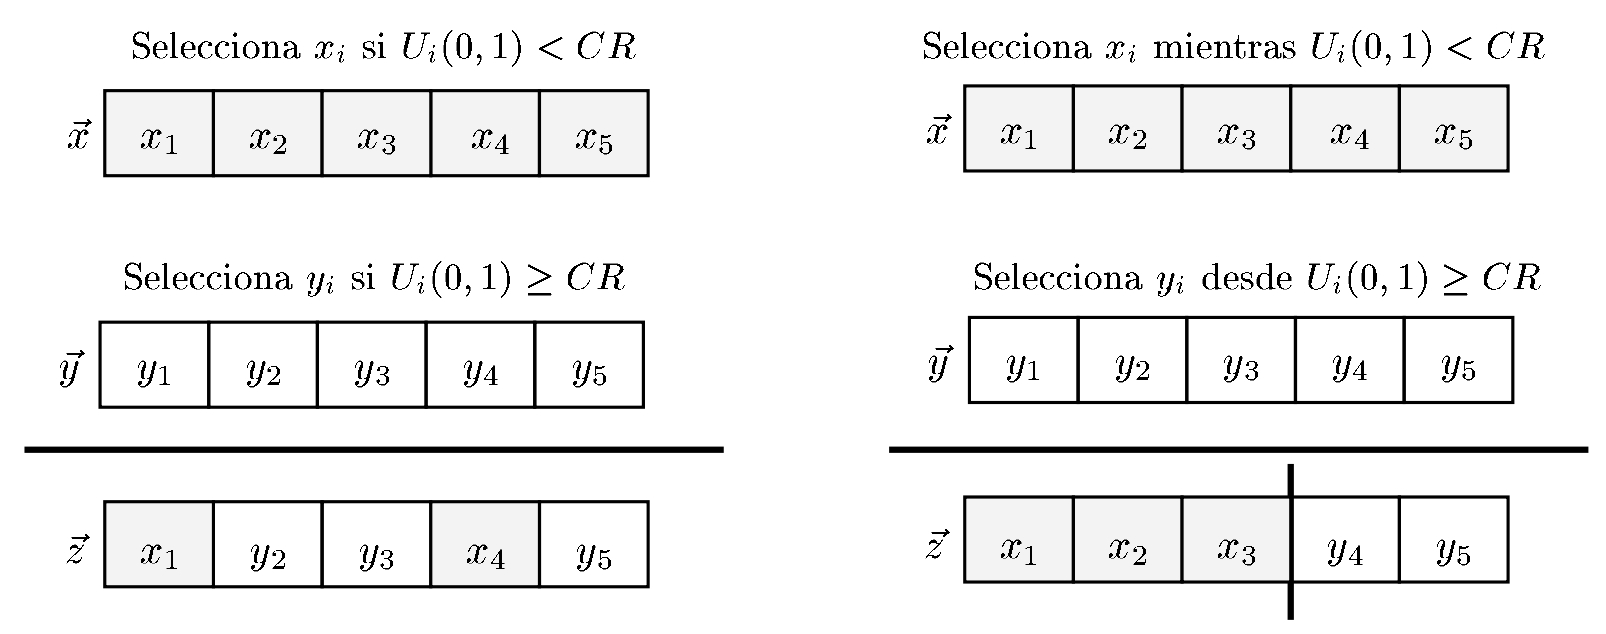
\includegraphics[keepaspectratio,width=11.5cm]{figuras/crucesBinonialExponencial.jpg}
\caption{Cruce discreto binomial (izquierda) y cruce discreto exponencial (derecha). Los
individuos $\mathbf{x}$ e $\mathbf{y}$ dan lugar a otro individuo $\mathbf{z}$.}
\label{diferencial1}
\end{figure}

\newpage
Definimos a continuación las variantes de la DE (la figura \ref{diferencial2} muestra un resumen de
las principales variantes):
\begin{itemize}
	\item Variantes con operador de cruce discreto (binomial o exponencial):
		\begin{itemize}
			\item \textit{DE/rand/1/bin}
			\item \textit{DE/rand/1/exp}
			\item \textit{DE/best/1/bin}
			\item \textit{DE/best/1/exp}
	   \end{itemize}
		Las variantes con \textit{rand} seleccionan el padre principal y un
		par de padres secundarios para calcular la mutación diferencial aleatoriamente. En
		contraste, las	variantes con \textit{best} utilizan la mejor solución
		de la población	como padre principal, y un par de individuos seleccionados
		aleatoriamente como padres		secundarios.
	\item Variantes con cruce aritmético:
		\begin{itemize}
			\item \textit{DE/current-to-rand/1}
			\item \textit{DE/current-to-best/1}
	   \end{itemize}
		La diferencia entre ellos es que el primero selecciona el padre principal y los
		padres secundarios de manera aleatoria en la población actual, mientras que el
		segundo utiliza la mejor solución de la población actual como padre principal, y los
		padres secundarios se eligen aleatoriamente.
			\item Variantes con cruce combinado aritmético discreto (similar a las anteriores pero
		utiliza cruce binomial):
		\begin{itemize}
			\item \textit{DE/current-to-rand/1/bin}
	   \end{itemize}
\end{itemize}
\newpage
\begin{figure}[!htp]
\centering
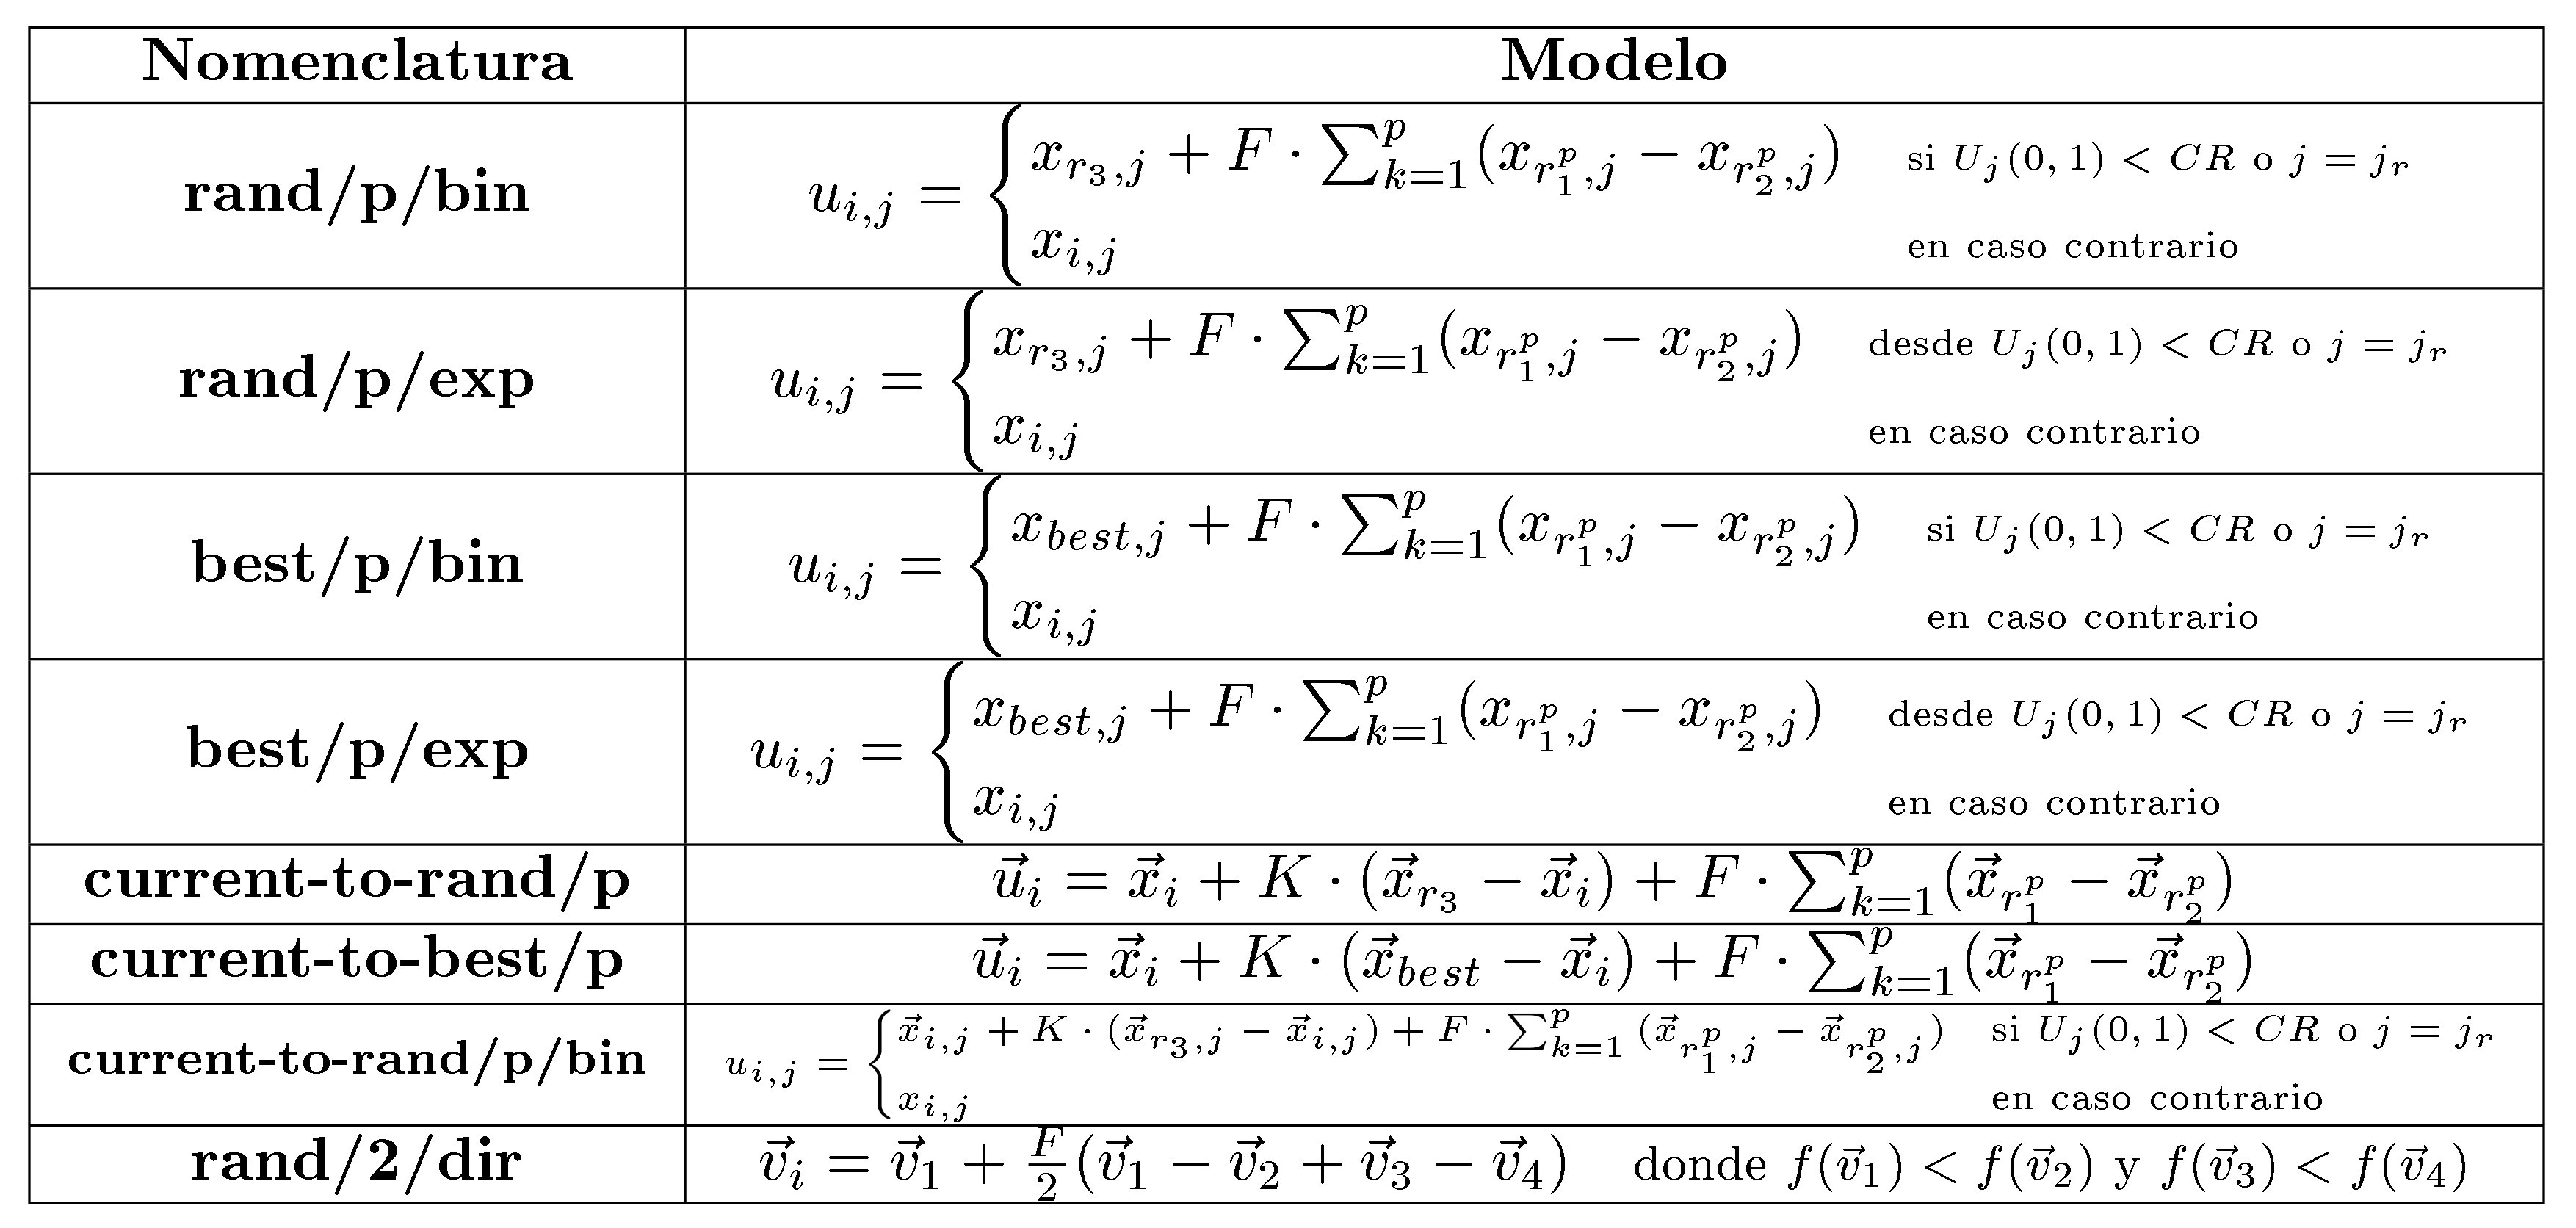
\includegraphics[width=13.2cm,height=9cm]{figuras/modelosDE.jpg}
\caption{Principales modelos de DE. $p$ es el número de pares de vectores que
conforman la diferencia, $j_{r}$ es un valor aleatorio generado en el
intervalo $\left[ 0,n\right]$, donde $n$ es el número de variables del problema.
$x_{r3}$ es el padre principal y $x_{r1}$ y $x_{r2}$ los padres
secundarios. $F$ y $K$ son valores de
escala, $u_{i}$ es el hijo creado y $x_{best}$ significa que se ha seleccionado como padre
principal el mejor individuo o solución de la población en una determinada generación,
\textit{bin} representa cruce binario y \textit{exp} cruce exponencial, y \textit{\textbf{dir}}
indica que se incluye información de alguna función de aptitud al cruce y a la mutación.}
\label{diferencial2}
\end{figure}
% \section{Evolución diferencial en redes neuronales artificiales mono-objetivo}
% \noindent Ning Guiying en \cite{Ning2007} propone un algoritmo basado en DE y llamado
%MDE
% (Modified Differential Evolution), en el que se optimizan los individuos iniciales con
%la
% regla $1/2$, introduciendo posteriormente una reorganización de la estrategia de
%evolución
% durante el período mutación. El MDE se utiliza para optimizar los pesos de ANNs
%multicapa
% hacia delante. MDE se compara con el algoritmo BP y con el algoritmo básico de DE,
% mostrando en los resultados finales que MDE tiene una alta calidad de convergencia
% global y mejora la precisión y la velocidad de convergencia de las ANNs.

% En \cite{Lahiri2008}, se utiliza un algoritmo de DE con ANNs, llamado ANN-DE, para
% optimizar reactores industriales catalíticos de óxido de etileno. En el proceso
% evolutivo del algoritmo se construye un modelo de ANN para correlacionar los datos del
% proceso que compone los valores de funcionamiento y de rendimiento de variables del
% reactor. Para la optimización de los pesos de la red se utiliza una algoritmo de
% gradiente y un conjunto de patrones de entrenamiento y generalización con tres
%variables, % que son obtenidas de la monitorización de una serie de reactores. Una vez se
%construye el % modelo de red se genera una serie de vectores aleatorios como población
%del proceso % evolutivo formados por posibles valores de las tres variables de entrada de
%los % reactores, es decir, se obtienen un número de conjuntos de condiciones de
%funcionamiento % que intentan maximizar la producción del reactor al aplicarlos a la ANN
%diseñada, la cual % muestra qué vectores de solución son mejores. Al final del proceso
%evolutivo, que posee % tanto cruce como mutación, se obtiene un conjunto de soluciones
%optimizadas  que se % vuelven a aplicar a la ANN para escoger finalmente la mejor.
\section{Evolución diferencial para optimización multi-objetivo utilizando el concepto de
dominacia de Pareto}
\noindent Para aplicar la estrategia de la DE a problemas multi-objetivo, hay que
modificar el esquema original \cite{Storn1997}, ya que el conjunto de soluciones de un
problema con múltiples objetivos no consiste en una sola solución (ver sección
\ref{multiobjetivo} del capítulo \ref{MOEANNs}).

Hay varios aspectos que se deben considerar para extender la DE a un problema de
optimización multi-objetivo:
\begin{itemize}
	\item ¿Cómo promover la diversidad de la población?
	\item ¿Cómo seleccionar o retener los mejores individuos, es decir, cómo realizar
	elitismo?
\end{itemize}

Para promover la diversidad hay que tener en cuenta el proceso de selección por medio de
mecanismos basados en alguna medida de calidad, la cual indique la cercanía entre los
individuos que forman la población. Las dos medidas de diversidad más usadas en
optimización multi-objetivo son:
\begin{description}
	\item[Distancia \textit{crowding} \cite{Deb2002}:] Esta medida da una idea de cómo de
agrupados están los vecinos de un determinado individuo en el espacio de la función
objetivo y hace que los frentes sean lo más uniformes posible, sin agrupar muchos
individuos en una
zona y dejar ninguno o muy pocos en otras. La distancia \textit{crowding} se estima en función
de la media de las caras de un cubo formado al tomar como vértices los vecinos más
cercanos a un
individuo $i$ (ver figura \ref{figuraCrowding} y el trabajo de K. Deb \cite{Deb2002} para más
información).
	\item[Compartición de aptitud o \textit{fitness sharing}:] Cuando un individuo
comparte valores de su función de aptitud con otros, ésta se degrada en proporción al número y
a la
proximidad de los individuos que lo rodean dentro de un determinado perímetro. La vecindad
de un individuo se define en términos de un parámetro llamado $\sigma_{share}$, que
indica el radio de la vecindad, a la cual se le llama nicho.
\cite{Golberg1989,Sareni1998}.
\end{description}

El lector puede obtener en \cite{Du2010} un estado del arte actualizado en métodos de
agrupamiento para obtener diversidad en ANNs.

\begin{figure}[!htp]
\centering
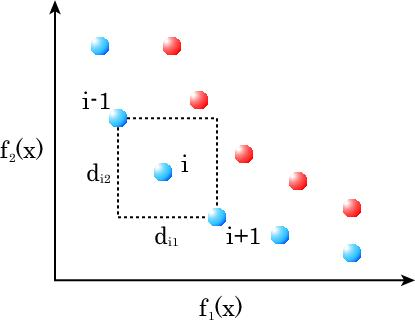
\includegraphics[keepaspectratio,width=8cm]{figuras/CrowdingDistance.jpg}
\caption{Cálculo de la distancia \textit{crowding}. Los puntos azules son soluciones de un mismo
frente.}
\label{figuraCrowding}
\end{figure}

Para promover el elitismo en optimización multi-objetivo se suele utilizar un archivo
externo, llamado población secundaria, que almacena los individuos no dominados
encontrados a lo largo de la búsqueda. Uno de los métodos más populares para seleccionar
los mejores individuos de una población formada por padres e hijos es la ordenación de
no dominados. Esta técnica se basa en el mecanismo de orden que se le da a los diferentes
individuos de una población en forma de niveles. Por ejemplo, en el nivel 1 estarán los
individuos no dominados. En el segundo nivel, estarán los individuos no dominados si no
se tienen en cuenta los del primer nivel, y así sucesivamente. Según Goldberg
\cite{Golberg1989}, para mantener una diversidad apropiada, la metodología de ordenación
de no dominados se debería usar en conjunción con alguna técnica de nichos como las
mencionadas anteriormente. El algoritmo NSGAII \cite{Deb2002} es un claro ejemplo de esto.

Existen varios trabajos interesantes que utilizan DE con MOEAs y aplicaciones en
\cite{Price2005,Chakraborty2008,Mezuza2008}.

\section{Evolución diferencial de Pareto con MOANNs}
\noindent En primer lugar vamos a considerar brevemente los artículos más interesantes
sobre el uso de DE para el diseño de ANNs mediante técnicas multi-objetivo basadas en el concepto de
de dominancia y óptimo de Pareto, y en los cuales nos hemos basado para la construcción
de un
nuevo MOEA basado en DE para el diseño de ANNs con unidades de base sigmoide.

El referente principal de este tipo de aplicaciones, usando una variación del algoritmo de
DE original \cite{Storn1997}, es H. Abbass, creador del algoritmo multi-objetivo PDE
(\textit{Pareto Differential Evolution}) \cite{Abbass2001-1,Abbass2002a}. En el algoritmo
PDE se utiliza un caso especial de la variante \textit{DE/current-to-rand/1/bin} con $K=0$
(ver penúltima fila de la figura \ref{diferencial2}), ya que el padre principal se utiliza
para la creación de un nuevo hijo y también para un tipo de cruce discreto. Los objetivos a
minimizar son el $MSE$ y la complejidad de la red.

El algoritmo trabaja como sigue: La población inicial se inicializa utilizando una distribución
Gaussiana de
media $0,5$ y de desviación típica $0,15$. Solamente las soluciones no dominadas se
retienen en la población para el cruce y las dominadas se eliminan. Se seleccionan tres
padres de manera aleatoria (uno de ellos como padre principal y también como solución
hija) para generar un nuevo hijo. Lo hijos se incluyen en la población solo si dominan al
padre principal, en caso contrario, se hace un nuevo proceso de selección. Si el número de
soluciones no dominadas excede un umbral, se adopta una métrica de distancia para eliminar
padres que están muy cercanos unos de otros (esto se puede ver como un procedimiento de
nichos en el cual la métrica de distancia es el radio del nicho). En esta aproximación, el
tamaño de paso $F$ se genera a partir de una distribución Gaussiana $N(0,1)$, y las
restricciones de frontera se preservan, ya sea mediante un cambio de signo si la variable
es $\leq 0$ o mediante restas repetitivas, restando 1 si es $\geq 0$, hasta que la
variable esté dentro de los límites permitidos. El algoritmo PDE también incorpora un operador de
mutación que se aplica con una determinada probabilidad, después del operador de cruce,
mediante la suma a cada variable de una pequeña perturbación aleatoria.

A partir de la aparición del algoritmo PDE, y casi en paralelo, Abbass desarrolla el algoritmo
MPANN (\textit{Memetic Pareto Artificial Neural Networks}) \cite{Abbass2001}, que es una
versión del PDE añadiéndole un algoritmo de LS basado en gradiente como es BP, con algunas
mejoras, para así aumentar la velocidad de convergencia. MPANN trata de obtener modelos
de ANNs que tengan buena capacidad de generalización sin aumentar demasiado el tamaño de
su arquitectura. Concretamente trata  de  minimizar  el $MSE$ y el número  de neuronas en  capa
oculta. MPANN evoluciona conjuntamente
la arquitectura y los pesos de la red y utiliza operadores cruce y mutación para la obtención de
los hijos, codificando cada ANN  en  un cromosoma  que  representa  la
estructura  y el  valor  de  los pesos. Otras  versiones  de MPANN  se
utilizan para problemas reales como la diagnosis del cáncer \cite{Abbass2002a},
diferenciándose del MPANN original en la incorporación de un operador de mutación, ya que
los algoritmos PDE y MPANN carecían de ello.

Otra variación del PDE es el algoritmo SPDE (\textit{Self-adaptive Pareto Differential
Evolution}) \cite{Abbass2002}, la cual adapta de manera automática las probabilidades de
cruce y mutación. Ambas probabilidades se heredan de los padres de la misma forma que se
realiza el cruce para las variables de decisión. Si las probabilidades de cruce y de mutación
no están entre $(0,1)$, se modifican automáticamente de acuerdo a unas reglas de
reparación. Al igual que se realizó una versión auto-adaptativa del PDE con el algoritmo
SPDE, Abbass propuso una versión auto-adaptativa del algoritmo MPANN, llamada SPANN
(\textit{Self-adaptive Pareto Artificial Neural Networks}) \cite{Abbass2003}.

Un algoritmo que se debe mencionar a pesar de que sea un algoritmo evolutivo
mono-objetivo con término de regularización es el de J. Illonen \cite{Jarno2003}, donde
se propone un estudio de la DE en el diseño de ANNs para encontrar el óptimo global de
un problema. El algoritmo utiliza el $MSE$ medio regularizado mediante la media de los pesos y los
sesgos para entrenar a las ANNs. Illonen compara su metodología con métodos basados en gradiente y
concluye que la DE puede ser más útil en el caso especial de algunas superficies de
error, pero que la inclusión de alguna metodología híbrida que utilice conjuntamente
optimización evolutiva e información basada en gradiente podría ser más beneficiosa.

En \cite{Yau2007}, se proponen una serie de experimentos utilizando el algoritmo
multi-objetivo PDE de Abbass para evolucionar ANNs aplicadas a juegos de inteligencia
artificial. La metodología propuesta contienes tres subsistemas: Un subsistema PDE canónico, un
subsistema que introduce coevolución en PDE con tres
configuraciones posibles (PCDE), y un subsistema también de coevolución con PDE usando un
archivo con tres configuraciones diferentes (PCDE-A). El primer subsistema se trata del algoritmo
PDE con operadores de cruce y mutación y sin LS. El segundo sistema introduce coevolución,
siendo la evaluación de cada individuo la principal diferencia con el algoritmo PDE. Para la
ejecución
del PCDE, cada ANN se compara con un número constante de ANNs elegidas al azar de la
población de la generación actual. Si la puntuación de la ANN es mayor o igual a la de su
oponente (elegidas al azar), recibirá una victoria. Por otra parte, la clasificación del
primer frente de Pareto (mediante el etiquetado de soluciones no dominadas) se basa en el
	número de victorias como criterio de evaluación principal. En el algoritmo PDCE-A, al
igual
que en PCDE, después de la puntuación de cada ANN se lleva a cabo un segundo computo.
Sin embargo, PCDE-A tiene un archivo extra que se utiliza para almacenar las soluciones
de Pareto cada 50 generaciones. En consecuencia, cada ANN se compara con un número
mínimo de ANNs elegidas al azar (sin repeticiones), a partir del archivo extra. Sólo si el
número de ANNs en el archivo es menor que el número mínimo exigido de oponentes elegidos al
azar, entonces la lista de oponentes se completa de ANNs elegidas al azar de la
población. Del mismo modo, una ANN recibirá una victoria si su puntación es mayor o
igual que la de su competidora. El número de victorias se utilizará como
criterio de evaluación principal para etiquetar las soluciones no dominadas para
el primer frente de Pareto. Este valor de evaluación será menor al depender del
etiquetado de las soluciones dominadas, a causa del conjunto acotado de
evaluadores. De la experimentación realizada con una serie de juegos de inteligencia
artificial, se concluye que los mejores resultados los obtiene el algoritmo PDE. El pobre
desempeño de los sistemas PCDE, incluso la versión que utilizan un archivo extra, en la
producción de una buena distribución de soluciones a lo largo del frente de Pareto, es una
prueba más de que los métodos co-evolutivos no son especialmente beneficiosos para la
síntesis de agentes inteligentes para juegos en la evolución de Pareto.

En \cite{Iorio2004} se propone un algoritmo llamado NSDE (\textit{Non-dominated Sorting
Differential Evolution}), que consiste en una modificación del algoritmo NSGAII
\cite{Deb2002}, al que se introduce DE con la variante \textit{DE/current-to-rand/1} (ver
sección \ref{variantes}) en el cruce y la mutación. NSDE se utiliza para resolver problemas
de rotación de funciones en el plano, atendiendo a dos funciones objetivo, una para cada
eje de coordenadas del plano basándose en los grados de rotación. El algoritmo NSDE se
compara con NSGAII en una serie de problemas de rotación, mostrando mejores
soluciones por el proceso de cruce y mutación realizado en este tipo de problemas.

A continuación exponemos algunos de los caminos futuros de la DE usando MOEAS.

\section{Caminos futuros en la evolución diferencial multi-objetivo}
\noindent Según se puede ver en \cite{Mezuza2008}, la DE debe tener en cuenta estas
futuras
mejoras:
\begin{description}
	\item[Diversidad:] A pesar de que la DE tiene una alta convergencia, no posee
suficiente robustez y tiene problemas para alcanzar el verdadero frente de Pareto,
pudiendo quedar atrapada en óptimos locales. Además parece que la DE tiene problemas para
crear un frente de Pareto homogéneo, con lo que se deberían aplicar alternativas de
diversidad cuando se utilice con problemas multi-objetivo.
	\item[Variantes:] A día de hoy no se sabe que variante de DE es mejor para problemas
multi-objetivo para alcanzar el verdadero frente de Pareto de menera más efectiva.
	\item[Operador de mutación:] Se deben tomar algunos nuevos criterios a la hora de
seleccionar pares de soluciones en el proceso de mutación que sean más efectivos
\cite{Iorio2006}. En este momento estamos estudiando la selección de soluciones utilizando
intervalos  de confianza asociados a las distribuciones de los mejores individuos de la población
\cite{Cruz2010}.
	\item [Adaptación de los parámetros:] Debe haber nuevas propuestas que no sean
solamente las autoadaptativas \cite{Abbass2002,Abbass2003} para optimizar los parámetros
CR y F.
	\item[Alternativas en la codificación:] DE se propuso para espacios se búsqueda
continuos, por lo que se debería buscar una alternativa de codificación que permita el
uso de la DE en problemas de optimización combinatoria.
	\item[Teoría:] Los estudios sobre la convergencia de las variantes de DE y análisis en
tiempo de ejecución, mejorarían la teoría actual.
 \end{description}

\section{El algoritmo MPANN}
\noindent A continuación exponemos el algoritmo MPANN \cite{Abbass2001} en su versión
adaptada al reconocimiento de diagnosis del cáncer \cite{Abbass2002a}. Ésta versión
se diferencia del algoritmo MPANN original en que incorpora un operador de mutación, del
cual
carecían los algoritmos PDE y MPANN originales. Además, tendremos en cuenta el algoritmo
NSGAII \cite{Deb2002}, que nos servirá de base para la creación de nuestro algoritmo MPDE para el
diseño de ANNs en multi-clasificación de patrones.

En la figura \ref{diferencial3}, se presenta el pseudocódigo del algoritmo
MPANN que comentamos a continuación:

El primer paso de MPANN es generar una población inicial al azar siguiendo una
distribución Gausiana $(0,1)$ (Paso 1).

Acto seguido, el algoritmo comienza su proceso evolutivo:

La primera acción (Paso 4) que tiene lugar al comienzo de una generación es la evaluación
de los individuos, en el caso de MPANN utilizando la minimización del $MSE$ y la
complejidad
de la red (número de neuronas en capa oculta). Una vez evaluados, se etiquetan los individuos no
dominados.

Si el número de individuos no dominados es menor que 3, se busca un individuo no dominado
de entre las soluciones que no están etiquetadas y se etiqueta como no dominado. Esto se
repite hasta que el número de no dominados sea igual a 3 (Paso 5).
\newpage
\begin{figure}[!htp]
\centering
\fbox{
	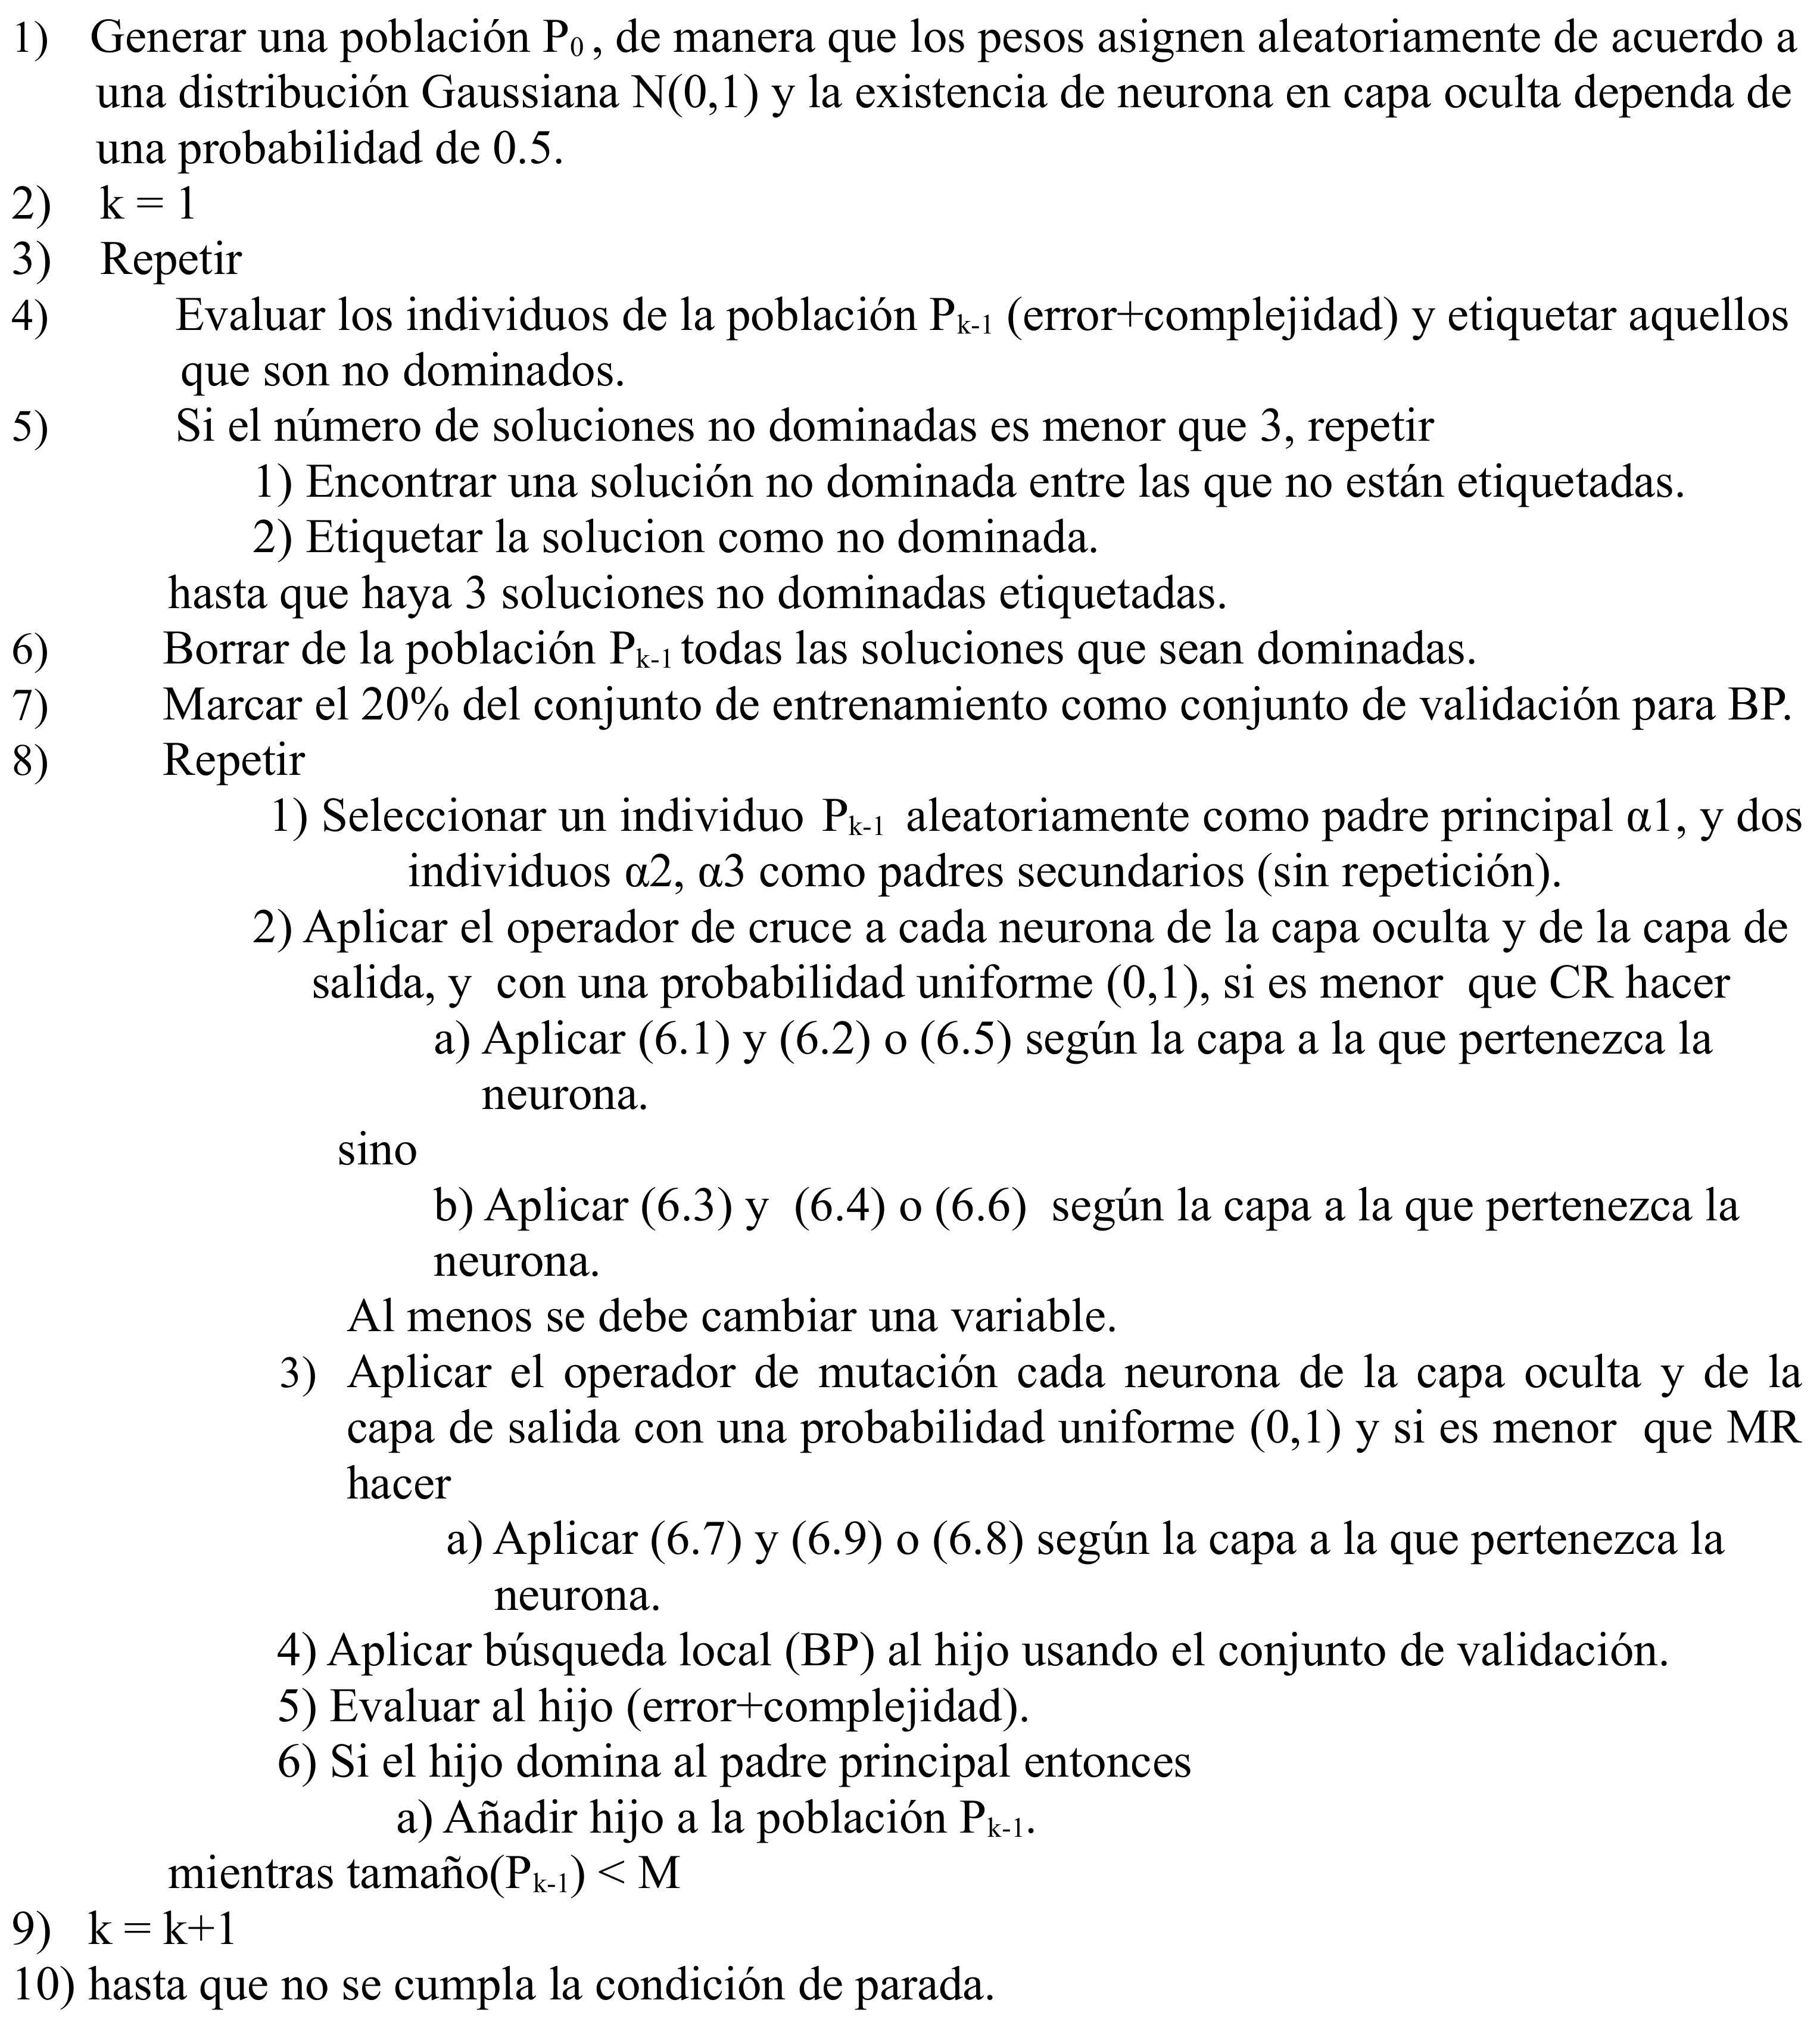
\includegraphics[keepaspectratio,width=12.2cm]{figuras/etapasMPANN.jpg}
}
\caption{Pseudocódigo del algoritmo MPANN.}
\label{diferencial3}
\end{figure}

Seguidamente (Paso 6), se eliminan todas las soluciones dominadas de la población.

A continuación (Paso 7), se marca un 20\% del conjunto de patrones de entrenamiento como
conjunto de validación para la LS.

El siguiente paso (Paso 8) es el más importante de todo el algoritmo, ya que se trata de
la generación de hijos. Este paso se repetirá hasta que la población alcance un tamaño
máximo, $M$, fijado de antemano.

La primera acción a realizar (Paso 8.1) es la selección aleatoria de tres
padres. Uno de ellos se etiqueta como padre principal $(\alpha_{1})$ y los otros dos
como secundarios $(\alpha_{2},\alpha_{3})$.

A continuación (Paso 8.2), tiene lugar la operación de cruce. En la operación de cruce se
calcula aleatoriamente una probabilidad uniforme en el intervalo $(0,1)$ para cada una de
las
neuronas de la capa oculta en conexión con la capa de entrada. Si el valor obtenido es menor que el
valor de $CR$ (\textit{Crossover Probability}), se aplican las expresiones (\ref{1}) y
(\ref{2}), donde  $w_{ih}^{hijo}$ se refiere, en el hijo, a los pesos asociados a cada una de las
neuronas de entrada, $i$, con cada una de las neuronas de la capa oculta, $h$. $\rho_{h}^{hijo}$ se
refiere a la existencia o no en la capa oculta de las neuronas del nuevo hijo. Todo este
proceso se hace para cada neurona de la capa oculta en conexión con la capa de entrada, siendo el
número máximo de neuronas ocultas prefijado al inicio del algoritmo.
\begin{equation}\label{1}
w_{ih}^{hijo} \leftarrow w_{ih}^{\alpha_{1}} +
N(0,1)(w_{ih}^{\alpha_{2}}-w_{ih}^{\alpha_{3}})
\end{equation}
\begin{equation}\label{2}
 \rho_{h}^{hijo} \leftarrow \left\lbrace
 \begin{array}{ll}
 1 & \mbox{si
$\rho_{h}^{\alpha_{1}}+N(0,1)(\rho_{h}^{\alpha_{2}}-\rho_{h}^{\alpha_{3}})\geq 0.5$} \\
 0 & \mbox{en otro caso}
 \end{array}
 \right.
\end{equation}

En el caso de que el valor aleatorio obtenido en el intervalo $(0,1)$ no sea menor que $CR$, se
aplican las expresiones (\ref{3}) y (\ref{4}).
\begin{eqnarray}
w_{ih}^{hijo} \leftarrow w_{ih}^{\alpha_{1}} \label{3} \\
\rho_{h}^{hijo} \leftarrow \rho_{h}^{\alpha_{1}} \label{4}
\end{eqnarray}

Una vez finalizada la operación de cruce para todas las neuronas de la capa oculta en
conexión
con la capa de entrada, es el turno de las neuronas de capa oculta en conexión con la capa de
salida. De nuevo se obtiene un valor aleatorio probabilístico uniforme en el intervalo $(0,1)$, y si
el valor obtenido es menor que el valor de $CR$, se aplica la expresión (\ref{5}), donde
$w_{ho}^{hijo}$ significa el peso asociado a la conexión que
va desde la neurona $h$ de la capa oculta hasta la neurona $o$ de la capa de salida  del nuevo hijo.
Esto se hace, al igual que antes, para todas las neuronas que haya en capa oculta en conexión con la
capa de salida.
\begin{equation}\label{5}
w_{ho}^{hijo} \leftarrow w_{ho}^{\alpha_{1}} +
N(0,1)(w_{ho}^{\alpha_{2}}-w_{ho}^{\alpha_{3}})
\end{equation}

En el caso de que el valor aleatorio obtenido en el intervalo $(0,1)$ no sea menor que $CR$, se
aplica la siguiente expresión:
\begin{equation}\label{6}
w_{ho}^{hijo} \leftarrow w_{ho}^{\alpha_{1}}
\end{equation}

Durante la operación de cruce, al menos una variable del hijo se debe modificar para que
sea distinto al padre principal.

A continuación se realiza la operación de mutación (Paso 8.3), calculándose
una probabilidad uniforme $(0,1)$ para cada una de las neuronas de capa oculta del hijo, tanto
las que están en conexión con la capa de entrada como las que están en conexión con la capa de
salida. Si el valor obtenido es menor que el valor de $MR$ (\textit{Crossover Probability}), se
aplican las expresiones (\ref{7}) y (\ref{9}), o la expresión (\ref{8}) si el cambio que se va a
producir es para una conexión de la  capa de oculta con la capa de entrada, o si
es para una conexión de la  capa de oculta con la capa de salida respectivamente. Si el valor
aleatorio obtenido es mayor que $MR$, no se hace la mutación. La nomenclatura que se sigue es la
misma que para la operación de cruce.
\begin{eqnarray}
w_{ih}^{hijo} \leftarrow w_{ih}^{hijo} +
N(0,\text{porcentaje mutación}) \label{7} \\
w_{ho}^{hijo} \leftarrow w_{ho}^{hijo} +
N(0,\text{porcentaje mutación}) \label{8}
\end{eqnarray}
\begin{equation}\label{9}
\rho_{h}^{hijo} \leftarrow \left\lbrace
\begin{array}{ll}
1 & \mbox{si
$\rho_{h}^{hijo}=0$} \\
0 & \mbox{en otro caso}
\end{array}
\right.
\end{equation}

Una vez realizadas las operaciones de cruce y mutación, se aplica al hijo resultante la LS (Paso
8.4), usando el algoritmo de retropropagación BP, aplicando el
conjunto de validación del paso 7.

Este hijo se evalúa y se añade a la población si presenta una relación de dominancia
con respecto al padre principal (Paso 8.5 y Paso 8.6)

Este proceso se repetirá a lo largo de las generaciones hasta que se cumpla la condición
de parada (Paso 10).

\section{El algoritmo MPDE}
\noindent A continuación exponemos nuestro algoritmo basado en DE para multiclasificación de
patrones usando el concepto de dominancia de Pareto. Dicho algoritmo se llama MPDE
(\textit{Memetic Pareto Differential Evolution}) \cite{Fernandez2009}. Nuestro procedimiento, al
igual que el algoritmo MPENSGAII descrito en el
capítulo \ref{MOEANNs}, evoluciona simultáneamente los pesos y la arquitectura de la red,
y se encarga de diseñar modelos de red para multi-clasificación de patrones.

MPDE obtiene diferentes conjuntos de clasificadores no dominados que presentan un buen
balance entre precisión y $MS$ (ver capítulo
\ref{medidasRendimiento}), que son los dos objetivos a optimizar.

La población de individuos está sujeta a operaciones de cruce y de mutación. En cuanto a la
codificación de los modelos de red, se sigue la misma codificación explicada en los algoritmos CBFEP
y MPENSGAII del capítulo \ref{evoMonoObjetivo} y \ref{MOEANNs} respectivamente.

MPDE está hibridado con un algoritmo de LS, y utiliza funciones de base sigmoides (SUs).

Para llevar a cabo un proceso de elitismo, MPDE se basa en algunos aspectos de NSGAII
\cite{Deb2002}, utilizando como característica más representativa el ordenamiento rápido
de no-dominados para la obtención del frente de Pareto.

Con respecto a la diversidad se utiliza la distancia \textit{crowding} de NSGAII, para el
caso en que haya que completar la población hasta alcanzar un número determinado de
individuos, y también una ecuación de cálculo de la distancia  de un individuo a los dos
vecinos más cercanos, la cual comentaremos en las siguientes secciones.

En cuanto a la variante de la DE, se trata de la variante \textit{DE/rand/1/bin}.
\newpage
\subsection{Funciones objetivo}
\indent Las funciones objetivo a optimizar con MPDE son las mismas que se utilizan con
MPENSGAII, $E$ y $MS$, ya que pensamos que un buen
clasificador
debería obtener un alto nivel de
precisión global, así como un aceptable nivel de clasificación para cada clase de un determinado
problema:
\begin{itemize}
\item \textbf{Objetivo 1:} La mínima sensibilidad de todas las clases de un problema, $MS$:
\begin{displaymath}
A_{1}\left( g,\mathbf{\Theta}\right) = MS(g)
\end{displaymath}
\item \textbf{Objetivo 2:} La entropía cruzada como medida de error global, $E$. Concretamente, como
función
de aptitud a la hora de evaluar un individuo se usará la siguiente expresión:
\begin{displaymath}
\label{aptitudNNEP}
A_{2}\left( g,\mathbf{\Theta}\right) =\frac{1}{1+E\left( g,\mathbf{\Theta}\right)},
\end{displaymath}
es decir, maximizar una transformación estrictamente decreciente de $E$.
\end{itemize}

A la hora de asignar una clase a una nueva observación se sigue el esquema ``1 de $Q$''
explicado en los algoritmos CBFEP y MPNESGAII.

\subsection{Operadores}
\noindent En cuanto a los operadores de cruce y mutación se utilizarán los mismos que los
del algoritmo MPANN, pero adaptados a nuestra representación.

Las expresiones (\ref{1}) a (\ref{6})
representan el operador de cruce y las expresiones (\ref{7}) a (\ref{9}) el
operador de mutación. El significado de la nomenclatura seguida es la misma que la
explicada en el algoritmo MPANN.

\subsection{Búsqueda local}
\noindent Como algoritmo de búsqueda local usamos el algoritmo iRprop+ utilizado con el
algoritmo MPENSGAII (ver sección \ref{rprop} del capítulo \ref{MOEANNs}). En la siguiente
sección se explica detalladamente cuándo se utiliza el algoritmo iRprop+ y se comenta
cada una de las etapas de nuestra metodología.

\subsection{Etapas y aspectos relevantes de MPDE}
\noindent En la figura \ref{diferencial3} se muestran las etapas del algoritmo MPDE, que
pasamos a comentar:

\begin{figure}[!htp]
\centering
\fbox{
	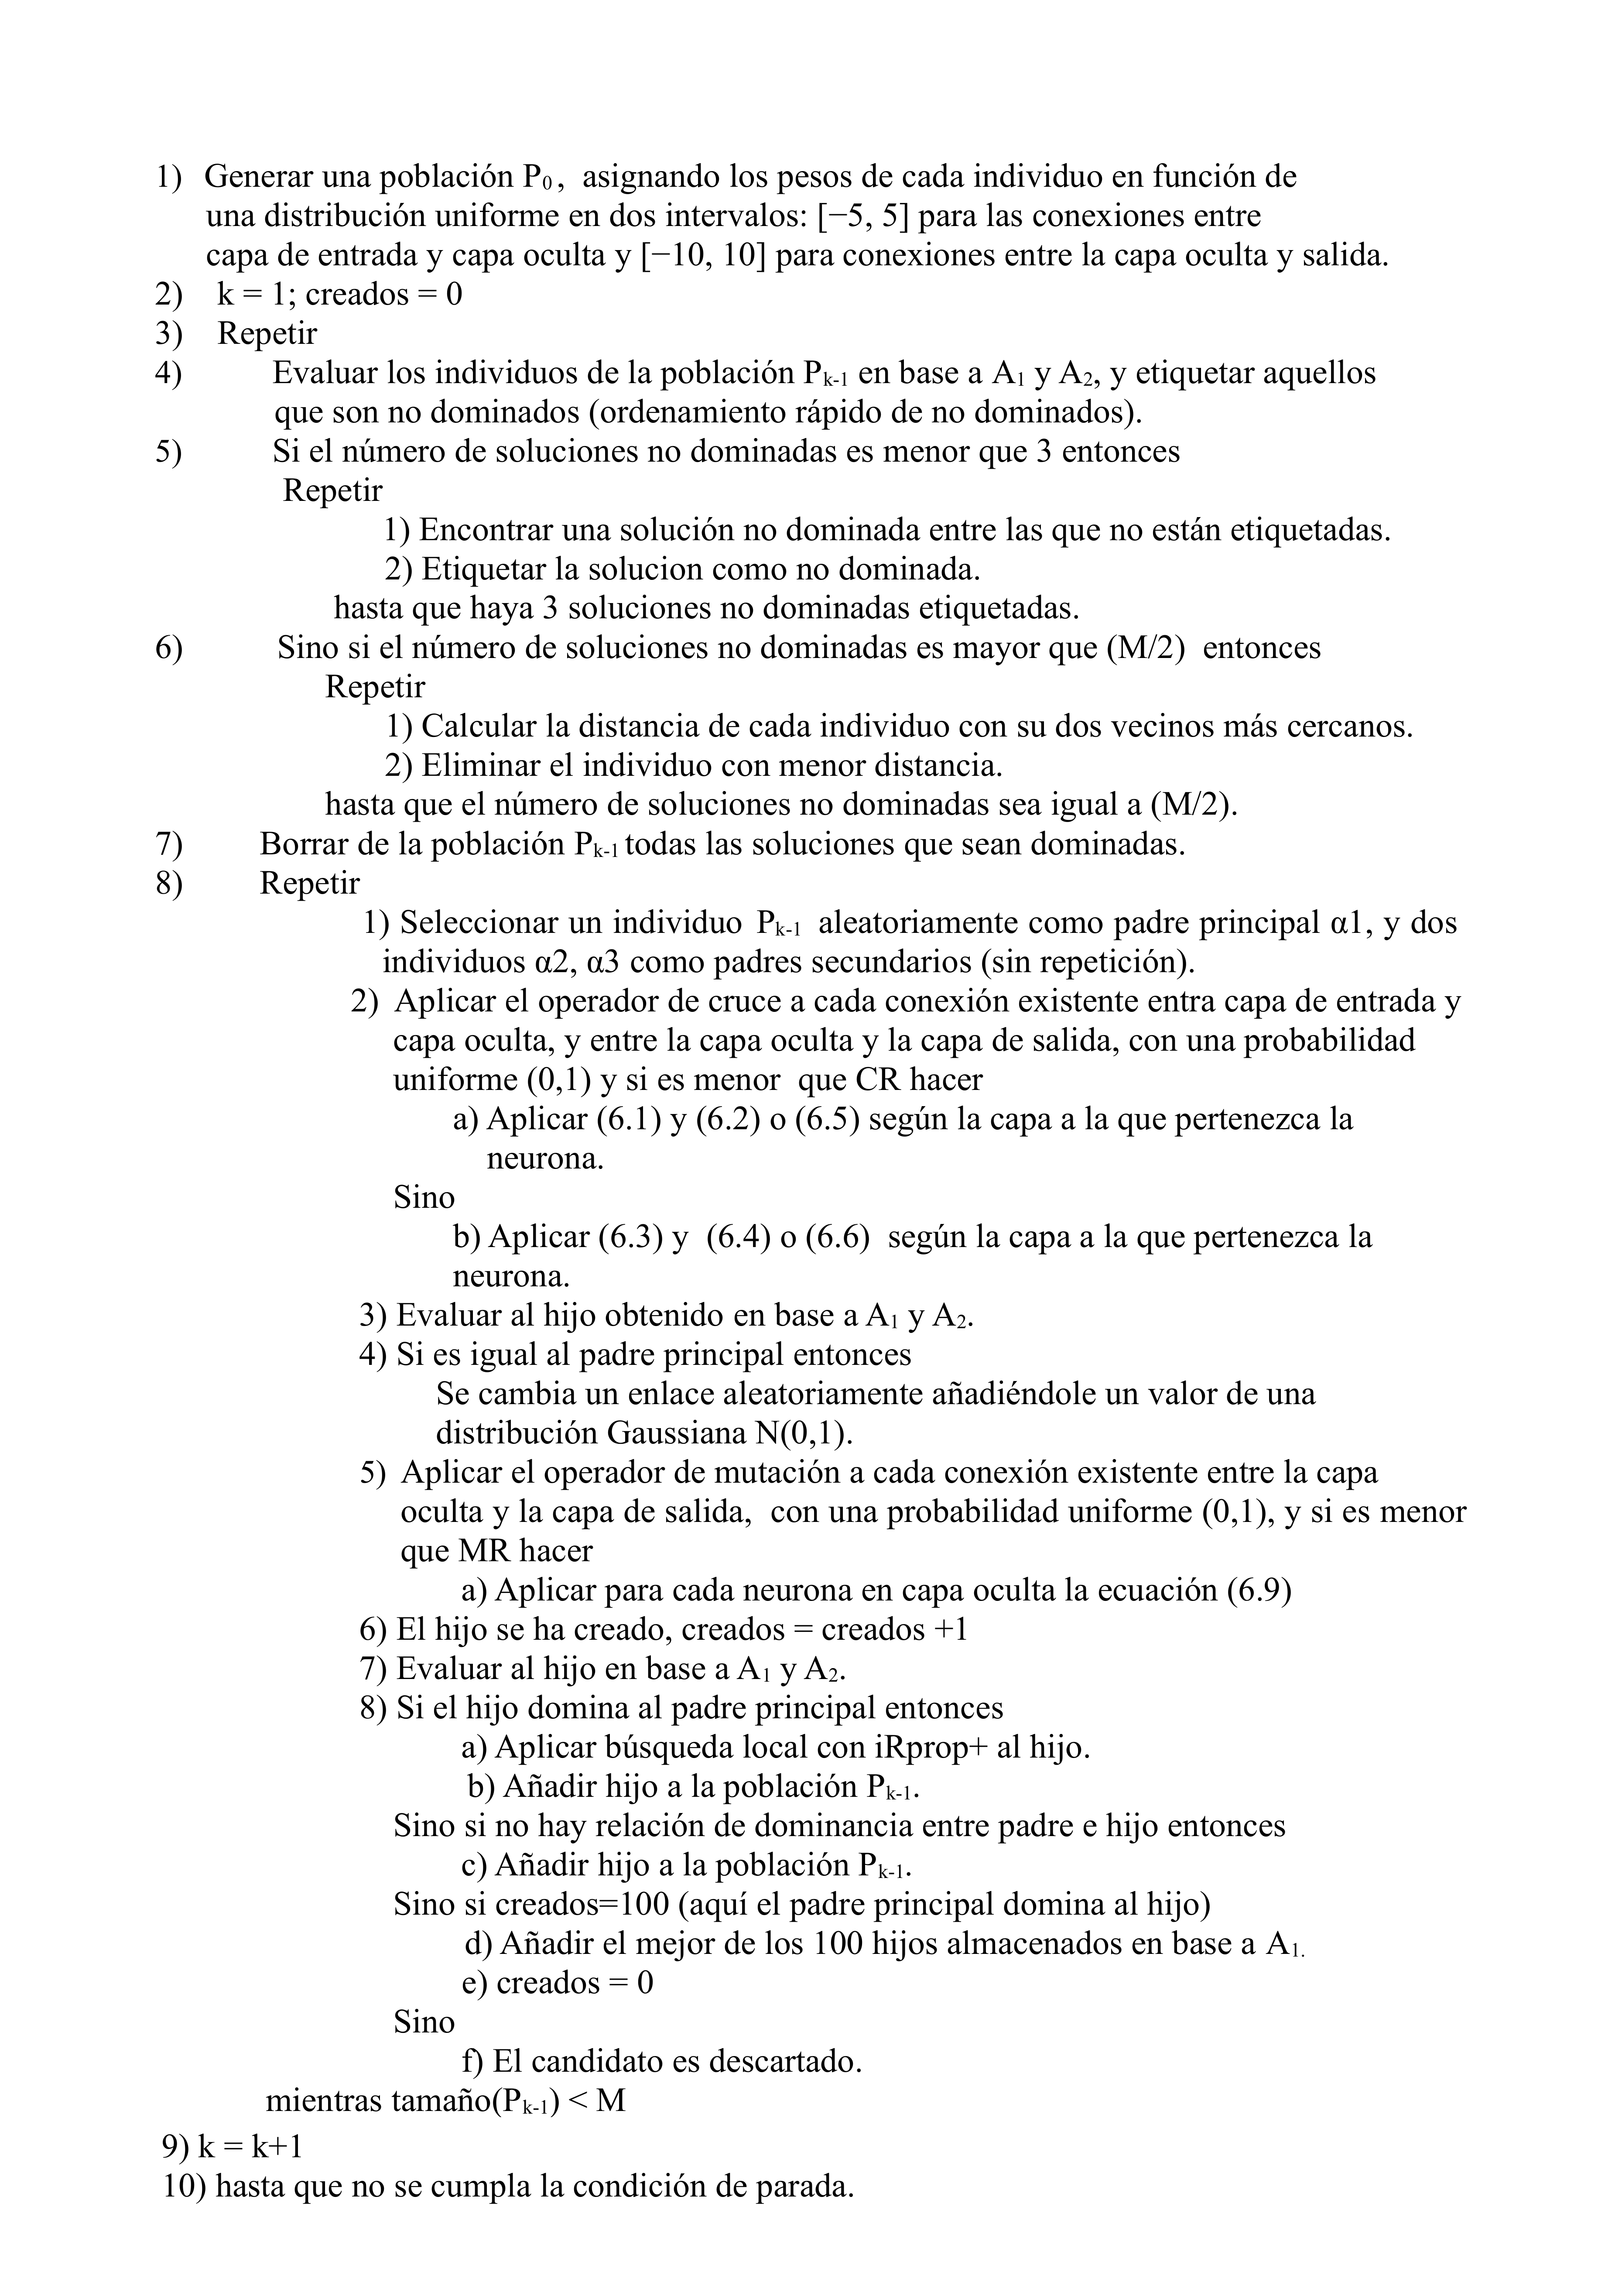
\includegraphics[keepaspectratio,width=12.2cm]{figuras/etapasMPDE.jpg}
}
\caption{Pseudocódigo del algoritmo MPDE.}
\label{diferencial4}
\end{figure}

El algoritmo comienza con la creación de una población de individuos tomados al azar,
siendo $M$ el tamaño de la población (Paso 1).

Empieza el proceso evolutivo hasta que se cumpla la condición de parada (Paso 3). Los
individuos se evalúan en base a las dos funciones objetivo que guían el algoritmo y se
realiza un ordenamiento rápido de no dominados equivalente al del algoritmo NSGAII
\cite{Deb2002}. Se etiquetan entonces aquellos que sean no dominados. (Paso 4)

Si el número de soluciones no dominadas es menor que 3 (Paso 5), entonces se repite el siguiente
proceso hasta que haya al menos 3 soluciones: Encontrar una solución no dominada
entre las que no están etiquetadas, en función del orden asignado en el ordenamiento
rápido de no dominados. En caso de empate en orden, se utiliza el valor de la distancia
\textit{crowding} de NSGAII (Paso 5.1) y se elige la solución con mayor distancia. A
continuación se
etiqueta el individuo escogido como no dominado (Paso 5.2).

Si el número de soluciones no dominadas ya era de al menos 3 individuos, se comprueba si
el número de soluciones es mayor que $M/2$ (Paso 6). Si es así, se calcula la distancia de
cada individuo a sus dos vecinos más cercanos (Paso 6.1), y se elimina el individuo con
menor distancia (Paso 6.2). El cálculo de la distancia viene dado por:
\begin{displaymath}
D(x)=\frac{(min\|x-x_{i}\|+min\|x-x_{j}\|)}{2}
\end{displaymath}
siendo $x$ el individuo al que se le va a calcular la distancia a sus dos vecinos más
cercanos, siendo estos $x_{i}$ y $x_{j}$. Esto nos permite mantener un mayor grado de
diversidad y que el algoritmo no quede estancado en el caso de que el número de
soluciones no dominadas sea cercano a $M$, ya que el tamaño de la población suele ser
pequeño, con lo que obtendríamos de una generación a otra muy pocos
individuos mejorados.

En el paso 7 se eliminan de la población actual todas las soluciones no etiquetadas, es
decir, las soluciones dominadas.

Se pasa ahora a completar la población actual para prepararla para la siguiente
generación hasta que el número de individuos sea igual a $M$ (Paso 8).

Primero se selecciona aleatoriamente un individuo como padre principal y otros dos como
padres secundarios, todo ello sin repetición, para que los 3 sean distintos (Paso 8.1).

A partir de esos tres individuos realizamos una serie de operaciones hasta
obtener un nuevo hijo que se añada a la población. En primer lugar aplicamos el operador
de cruce a partir del padre principal y a partir de los padres secundarios, con una
probabilidad de cruce uniforme designada como $CR$ (Paso 8.2). El hijo que se obtenga, tendrá
características de los tres padres.

El hijo obtenido se evalúa en base a las dos funciones objetivo que guían al algoritmo
(Paso 8.3), y si el individuo es igual al padre porque no se hayan producido cambios con
las operaciones realizadas anteriormente, se le fuerza a cambiar aleatoriamente un enlace,
añadiéndole un valor de una distribución Gaussiana $N(0,1)$ (Paso 8.4).

A continuación, se aplica al hijo el operador de mutación en cada una de sus
neuronas de la capa oculta (Paso 8.5). Al comenzar el algoritmo se establece un número
máximo de neuronas como en el algoritmo MPENSGAII (ver capítulo \ref{MOEANNs}). Para el
total del máximo de neuronas, si la neurona $i$ existe se elimina, y si no, se añade,
estableciendo enlaces y pesos de la misma forma que la mutación añadir neurona del
algoritmo MPENSGAII. Todo ello aplicando la mutación con una probabilidad determinada.

Cuando el nuevo hijo se ha creado, aumentamos en 1 el valor de una
variable llamada ``creados'', que nos servirá, en un momento dado de la evolución. Concretamente
cuando se hayan creado muchos hijos y ninguno de ellos por las circunstancias que se explican a
continuación se pueda añadir a la población actual (Paso 8.6).

Evaluamos al hijo en base a las dos funciones objetivo que guían a MPDE (Paso 8.7).

Si el hijo domina al padre principal se le aplica la LS con el algoritmo iRprop+ y se añade a
la población actual (Paso 8a y 8b). En caso contrario, si no hubiera relación de dominancia entre
padre e hijo, también se añade el hijo a la población actual (Paso 8c). En caso contrario, si el
padre principal domina al hijo, se comprueba si $creados=100$. En ese caso se elige el mejor de los
100 hijos almacenados, en base a la función objetivo $A_{1}$, y la variable creados se establece a
$0$ (Paso 8d y 8e). Sino se produce nada de lo anterior, el candidato es descartado (Paso
8f). El paso 8 se repite entero hasta completar el tamaño de la población que se establece en la
variable $M$.

Cuando se complete el tamaño de la población, ésta queda preparada para la siguiente
generación (Paso 9), y el proceso evolutivo continúa hasta que se cumpla la condición de
parada, que en nuestro caso es un número determinado de generaciones (Paso 10).


\subsection{Diferencias con el algoritmo MPANN}\label{diferencias}
\noindent Las diferencias fundamentales con respecto al algoritmo MPANN \cite{Abbass2002a} son las
siguientes:
\begin{itemize}
	\item El operador de cruce que nosotros utilizamos, también calcula aleatoriamente una
probabilidad uniforme en el intervalo $(0,1)$, y si el valor obtenido es menor que
el	valor de $CR$ no se aplica el operador. La diferencia está en que nuestro método no aplica el
valor de probabilidad obtenido aleatoriamente a todos los enlaces y neuronas de la capa oculta, sino
que utilizamos un nuevo valor aleatorio dentro del intervalo uniforme definido para
cada neurona y no para la capa oculta entera, como en el caso de MPANN. En este caso, nuestro
operador de cruce es menos agresivo con los cambios en las ANNs, ya que en alguna ocasión puede
que el valor aleatorio obtenido a partir de una probabilidad uniforme no sea menor que $CR$, con lo
que la neurona que se esté tratando es ese momento no cambia.
	\item La probabilidad de mutación $MR$, también se utiliza de manera independiente, al igual que
en el cruce, para cada neurona, y no para la capa oculta entera, como en el caso del algoritmo
MPANN.
	\item La manera en que  se añaden los individuos a la población en el algoritmo MPANN
	(solo los que dominan al padre principal), hace que el algoritmo pueda quedar estancado durante
	un buen número de generaciones (se ha comprobado experimentalmente) hasta que se pueda añadir
	un nuevo hijo. Nosotros añadimos individuos de una manera más ``relajada'', de
	manera que hijos que no dominen al padre principal tienen la opción de añadirse a la
	población. De esta manera también se reduce el coste computacional sin disminuir la
	calidad de los resultados.
\end{itemize}

\subsection{Diseño experimental}
\noindent Para analizar el rendimiento de MPDE hemos utilizado 6
conjuntos de datos del repositorio de la UCI \cite{UCI2007}.

En la tabla \ref{tabla1MPDE} se muestran las características de cada
conjunto: Número total de patrones por cada
conjunto de datos, número de patrones en entrenamiento y en generalización, número de
variables de entrada, número de clases, número total de patrones por clase y valor de $p^*$.

\begin{table}[htb!]
\scriptsize
\caption{Características de los conjuntos de datos de la UCI.}
\label{tabla1MPDE}
\centering
\tabcolsep 1pt
\begin{tabular}{c c c c c c p{2.5cm} c}
\hline
\rowcolor[rgb]{0.70,0.85,1}\textbf{Conjunto} & \textbf{Patrones} &
\textbf{Patrones} & \textbf{Patrones} &
\textbf{Variables} & \textbf{Clases} &
\textbf{Patrones} & $\mathbf{p^{*}}$ \\
\rowcolor[rgb]{0.70,0.85,1} & & \textbf{entrena.} & \textbf{generaliz.} & \textbf{de
entrada} & & \textbf{por clase} & \\ \hline
% \multicolumn{8}{>{\columncolor[rgb]{0.70,0.85,1}}c}{Dos clases} \\ \hline
\rowcolor[rgb]{0.86,0.94,1}Autos & 205 & 152 & 53 & 72 & 6 & 67-3-22-54-32-27 & 0.0188 \\
\rowcolor[rgb]{0.86,0.94,1}Balance & 625 & 469 & 156 & 4 & 3 & 288-49-288 & 0.0641 \\
\rowcolor[rgb]{0.86,0.94,1}BreastC & 286 & 215 & 71 & 15 & 2 & 201-85 & 0.2957 \\
\rowcolor[rgb]{0.86,0.94,1}HeartStatlog & 270 & 202 & 68 & 13 & 2 & 150-120 & 0.4411 \\
\rowcolor[rgb]{0.86,0.94,1}Newthyroid & 215 & 161 & 54 & 5 & 3 & 150-35-30 & 0.1296 \\
\rowcolor[rgb]{0.86,0.94,1}Pima & 768 & 576 & 192 & 8 & 2 & 500-268 & 0.3489 \\ \hline
\end{tabular}
\end{table}

El diseño experimental consiste en una partición estratificada del conjunto de datos con $3n/4$
patrones para
el conjunto de entrenamiento y $n/4$ patrones para el conjunto de generalización, siendo $n$ el
tamaño del conjunto.

El proceso de obtención de resultados es el mismo que el utilizado con MPENSGAII (ver
sección \ref{disenio} del capítulo \ref{MOEANNs}). Una vez se forma el frente de Pareto
se utilizan dos estrategias de selección
automática de individuos, el mejor modelo en $E$ y el mejor modelo en $MS$
(extremos del frente de Pareto). En cada ejecución del algoritmo (hacemos 30, dado que el proceso
de entrenamiento de la red es estocástico), una vez que tenemos el frente de Pareto de la última
generación del proceso evolutivo, se escogen los
extremos del frente en entrenamiento. Esto es, el mejor individuo en $E$, y el
mejor individuo en $MS$. A estos individuos se les llamamos individuo
$EI$, para el primer caso, e individuo $MSI$, para el segundo. Cuando tenemos los
individuos del paso anterior calculamos su valor de $C$ y de $MS$, sobre el conjunto
de generalización. De esta manera, tenemos para los extremos del frente dos pares de valores,
$\displaystyle EI=(C_{EI},MS_{EI})$ y $\displaystyle MSI=(C_{MSI},MS_{MSI})$ de una ejecución de las
30 realizadas.

Al repetirse el proceso anterior 30 veces obtenemos la media y la desviación
típica de los dos pares de valores para los individuos $EI$ y $MSI$, es decir,
$\displaystyle \overline{EI}=(\overline{C}_{EI},\overline{MS}_{EI})$ y
$\displaystyle \overline{MSI}=(\overline{C}_{MSI},\overline{MS}_{MSI})$, de forma que la
primera expresión muestra el rendimiento medio obtenido teniendo en cuenta solo los
mejores individuos en $E$, mientras que la segunda expresión muestra el rendimiento
medio teniendo en cuenta solo los mejores individuos en $MS$. A la manera
de obtener automáticamente el rendimiento medio teniendo en cuenta los mejores individuos
en $E$ (parte superior del frente) le hemos llamado MPEDEE, a y la forma de obtener el
rendimiento medio teniendo en cuenta los mejores individuos en $MS$ (parte inferior del
frente) la hemos llamado MPDES.

La probabilidad de cruce se estableció a $CR=0.8$ y la de mutación a $MR=0.1$, que es la
adoptada por Abbass en MPANN, y el tamaño de la población se estableció como $M=25$.

Para iRprop+, los parámetros adoptados son $\eta^{-}=0.5$ (tamaño de paso para el factor
de decremento), $\eta^{+}=1.2$ (tamaño de paso para el factor de incremento),
$\bigtriangleup_{0} =0.0125$ (valor inicial de tamaño de paso para los pesos,
$\bigtriangleup_{ij}$),  $\bigtriangleup_{min} =0$ (tamaño
mínimo de paso para los pesos), $\bigtriangleup_{max} =50$ (tamaño máximo de paso
para los pesos), $Epochs=5$ (número de épocas para la optimización local).

\subsection{Resultados}
\noindent Hemos comparado MPDE con nuestro algoritmo MPENSGAII y con la metodología SVM, a
partir del algoritmo SMO que proporciona Weka \footnote{http://www.cs.waikato.ac.nz/ml/weka/}
\cite{Witten2005}.

La tabla \ref{tabla2MPDE} presenta los valores de media y desviación típica para $C$ y
$MS$ obtenidos de los mejores modelos en $E$ en cada ejecución. Observar que en Balance y
Breast Cancer, el algoritmo MPDES obtiene los mejores valores en $MS$, encontrándose muy
cercano al algoritmo MPENSGAII en valores de $C$. En Autos, el mejor resultado en $C$ lo
obtiene MPDEE, pero el mejor resultado en $MS$ lo consigue el algoritmo MPENSGAIIS. En Newthyroid,
MPDE obtiene los mejores valores en $MS$ y $C$, y en Pima y Heart Statlog, MPDES obtiene
los mejores valores en $MS$, y muy similares en $C$ a los que obtiene MPENSGAIIE.

\begin{table}[!htb]
\tiny
\caption{Resultados estadísticos para MPDE, MPENSGAII y SVM en media y desviación típica
sobre el conjunto de generalización para $C$ y $MS$.}
\label{tabla2MPDE}
\centering
\tabcolsep 2pt
\renewcommand{\arraystretch}{1.2}
\begin{tabular}{llccllcc}
\hline
\rowcolor[rgb]{0.70,0.85,1}\textbf{Conjunto} & \textbf{Algoritmo} & \textbf{C(\%)} &
\textbf{MS(\%)} & \textbf{Conjunto} & \textbf{Algoritmo} & \textbf{C(\%)} &
\textbf{MS(\%)} \\ \hline
\rowcolor[rgb]{0.86,0.94,1}Autos & MPDEE & \textbf{68.79$\pm$5.59} & 28.75$\pm$21.40 &
Balance & MPDEE & 91.43$\pm$1.01 & 54.36$\pm$26.25 \\
\rowcolor[rgb]{0.86,0.94,1}& MPDES & 64.15\textit{$\pm$}5.63 &
12.26\textit{$\pm$}20.54\textbf{} &  & MPDES & 91.41$\pm$1.53 & \textbf{87.42$\pm$4.32}
\\
\rowcolor[rgb]{0.86,0.94,1}& MPENSGAIIE & \textit{66.67$\pm$4.07} &
\textit{39.64$\pm$14.92} &  & MPENSGAIIE & \textbf{94.01}$\pm$1.52\textbf{} &
42.66$\pm$17.00 \\
\rowcolor[rgb]{0.86,0.94,1}& MPENSGAIIS & 66.04\textit{$\pm$}4.78\textbf{\textit{}} &
\textbf{42.28\textit{$\pm$}10.98}\textit{\underbar{}} &  & MPENSGAIIS &
\textit{92.47$\pm$2.16} & \textit{83.72$\pm$8.19} \\
\rowcolor[rgb]{0.86,0.94,1}& SVM & 67.92 & 0.00 &  & SVM & 88.46 & 0.00 \\ \hline
\rowcolor[rgb]{0.86,0.94,1}BreastC & MPDEE & \textit{67.27$\pm$2.71} & 38.09$\pm$11.59 &
Newthy & MPDEE & \textit{96.66$\pm$2.02} & \textit{81.42$\pm$10.74} \\
\rowcolor[rgb]{0.86,0.94,1} & MPDES & 65.39$\pm$3.40\textbf{} & \textbf{57.04$\pm$7.01} &
& MPDES & \textbf{96.66$\pm$1.84} & \textbf{81.64$\pm$9.76} \\
\rowcolor[rgb]{0.86,0.94,1}& MPENSGAIIE & \textbf{69.34$\pm$2.30} & 28.88$\pm$9.09 &  &
MPENSGAIIE & 95.12$\pm$2.30\textbf{} & 74.81$\pm$10.07 \\
\rowcolor[rgb]{0.86,0.94,1} & MPENSGAIIS & 63.99$\pm$3.10 & \textit{53.08$\pm$6.57} &  &
MPENSGAIIS & 95.55$\pm$2.15 & 75.07$\pm$10.66\textit{} \\
\rowcolor[rgb]{0.86,0.94,1}& SVM & 64.79 & 23.81 &  & SVM & 88.89 & 55.56 \\ \hline
\rowcolor[rgb]{0.86,0.94,1}Pima & MPDEE & \textit{78.59$\pm$1.59} & 61.94$\pm$4.10 &
HeartStlg & MPDEE & 76.17$\pm$1.41 & 61.11$\pm$2.20 \\
\rowcolor[rgb]{0.86,0.94,1}& MPDES & 77.11$\pm$2.20\textbf{\textit{}} &
\textbf{73.12$\pm$2.98} &  & MPDES & \textit{76.27$\pm$1.57} & \textbf{63.66$\pm$2.37} \\
\rowcolor[rgb]{0.86,0.94,1}& MPENSGAIIE & \textbf{78.99$\pm$1.80} & 60.44$\pm$2.59 &  &
MPENSGAIIE & \textbf{78.28$\pm$1.75}\textit{} & 61.88$\pm$2.08\textit{} \\
\rowcolor[rgb]{0.86,0.94,1}\textbf{} & MPENSGAIIS & 76.96$\pm$2.08 &
\textit{72.68$\pm$3.06} &  & MPENSGAIIS & 77.5$\pm$1.73 & \textit{62.66$\pm$2.38}\textbf{}
\\
\rowcolor[rgb]{0.86,0.94,1} & SVM & 78.13 & 50.75 &  & SVM & 76.47 & 60.00 \\ \hline
\multicolumn{8}{l}{Los mejores resultados se muestran en \textbf{negrita} y los segundos
mejores resultados se muestran en \textit{cursiva}.}\\
\end{tabular}
\end{table}

Como ejemplo gráfico en la figura \ref{figuraBalance}, presentamos los resultados obtenidos por
el algoritmo MPDE en el conjunto de datos Balance, y al igual que en el caso de MPENSAII (ver
sección \ref{resultadosMPENSGAII} del capítulo \ref{MOEANNs}), están divididos en gráficos de
entrenamiento $(A_{1},A_{2})$, y en gráficos de generalización $(A_{1},C)$.

En nuestra opinión, el uso de la DE junto con métodos de LS usando $E$ y $MS$ como
objetivos
a optimizar, puede ser un nuevo punto de vista para tratar problemas multi-clase en clasificación,
con resultados muy prometedores.

En el siguiente capítulo se expone una aplicación realiza con el algoritmo MPENSGAII que
estudiamos y detallamos en el capítulo \ref{MOEANNs}, concretamente una aplicación sobre
microbiología predictiva \cite{Valero2009}.

\begin{figure}[!htb]
\centering
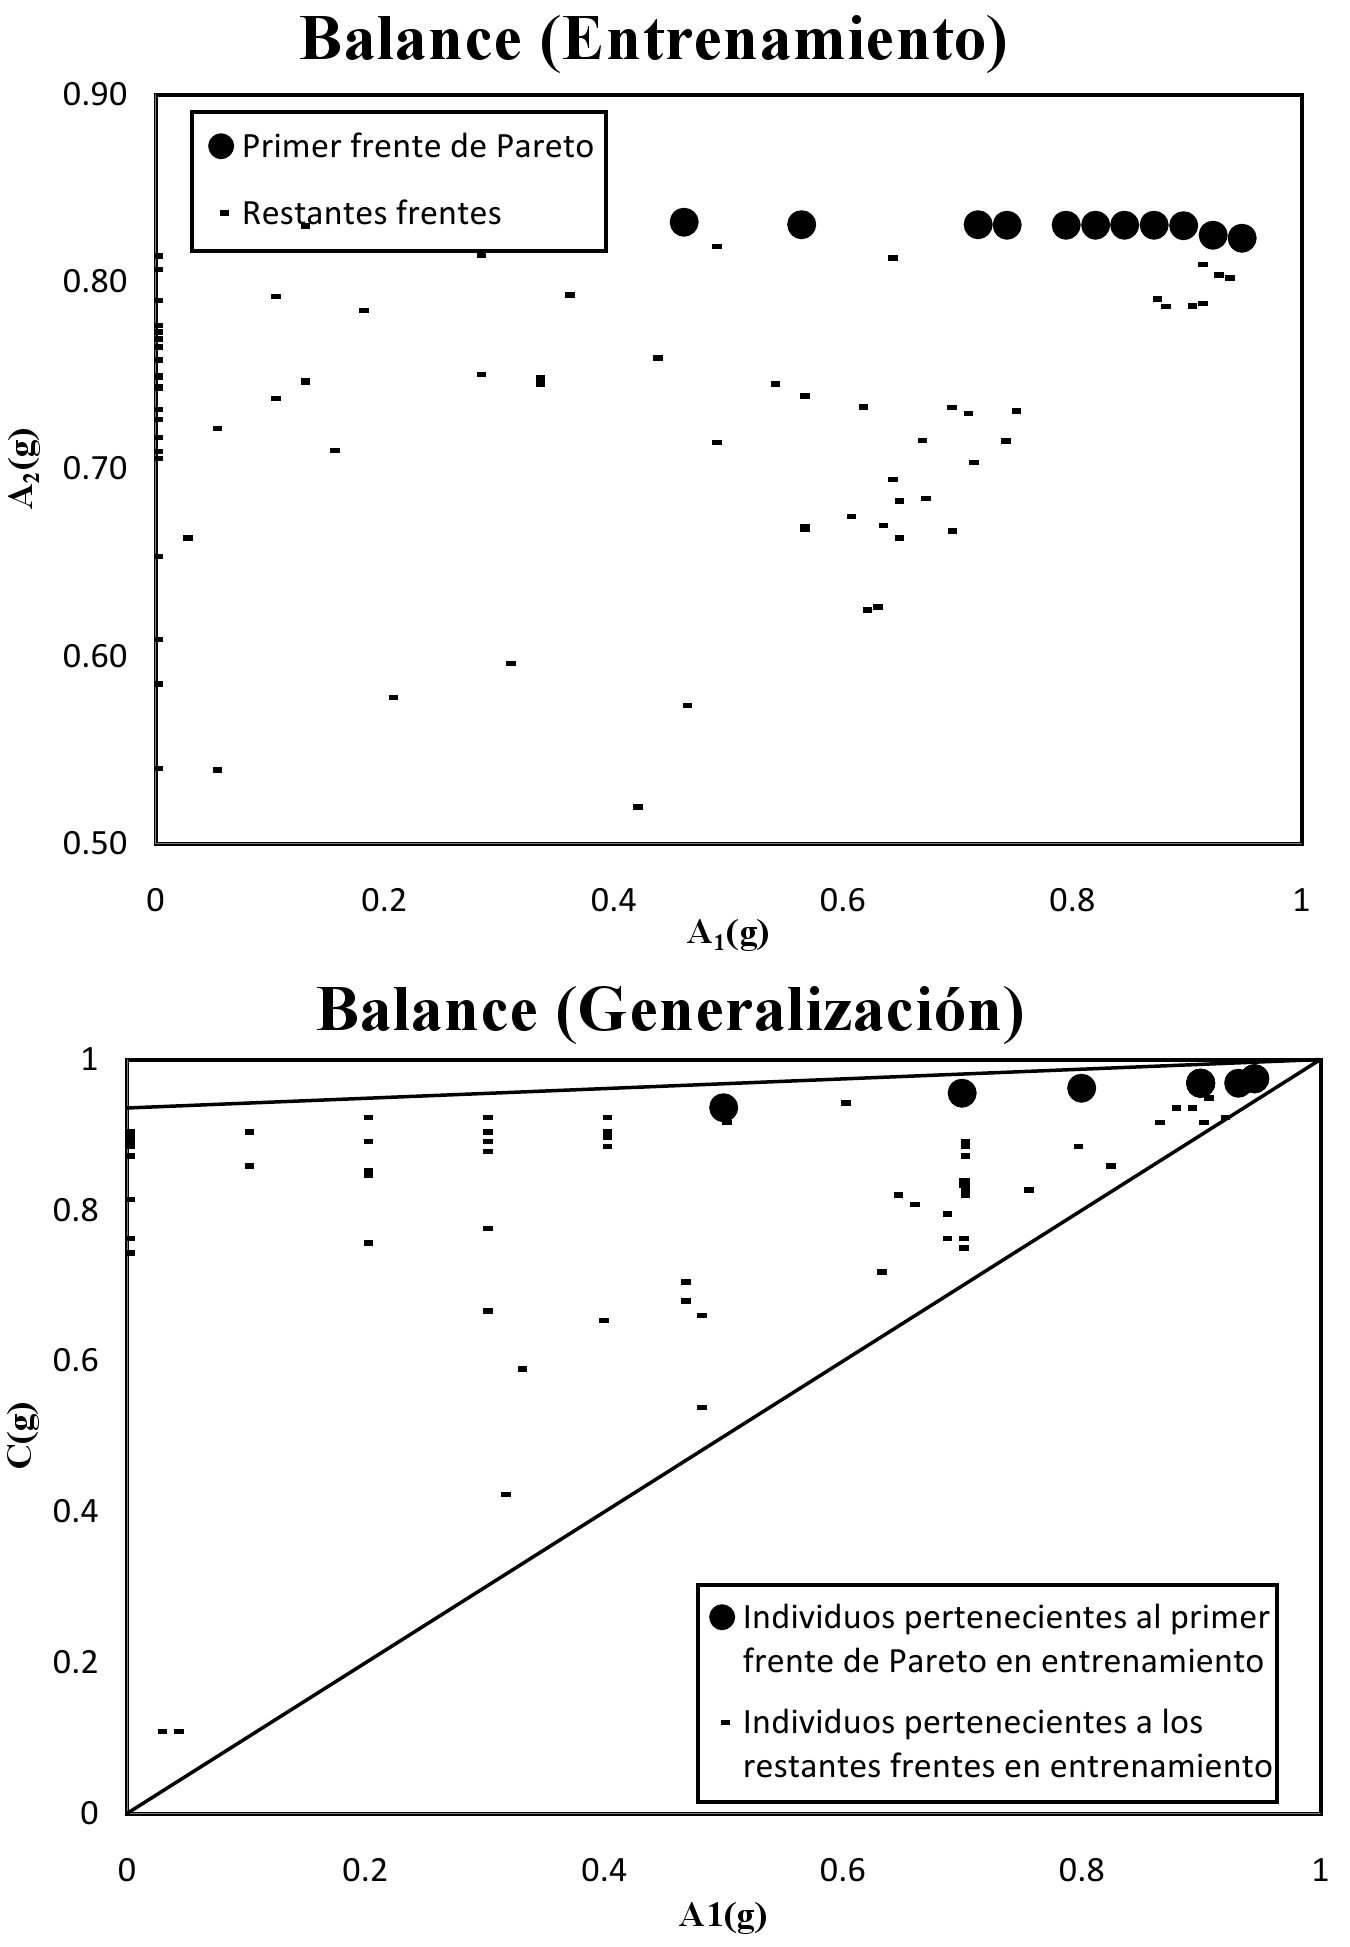
\includegraphics[keepaspectratio, width=8cm]{figuras/ejemploBalanceMPDE.jpg}
\caption{Frente de Pareto en entrenamiento $(A_{1},A_{2})$, y valores asociados a\\
$(A_{1},C)$ en generalización para el conjunto de datos Balance.}
\label{figuraBalance}
\end{figure}
\paginavaciacompleta
% \section{Introducción a los intervalos de confianza}
%
% \subsection{Intervalos de confianza aplicados a la evolución diferencial con redes}
% \noindent Aquí se hablará de los intervalos de confianza, las distintas normas y se
% pondrá HPDE con y sin intervalos de confianza.
% Se podría hacer también una breve comparación con resultados obtenidos sin intervalos de
% confianza para ver si se mejora.
%
% Velazquez tesis, pag 96
% \chapter{El algoritmo HPDCI}
%
% \section{Funciones objetivo}
%
% \section{Operadores}
%
% \section{iRprop+ como búsqueda local}
%
% \section{Etapas y aspectos relevantes de HPDE}
%
% \section{Resultados}